%%%%%%%%%%%%%%%%%%%%%%%%%%%%%%%%%%%%%%%%%%%%%%%%%%%%%%%%%%%%%%%%%%%%%%%%%%%%%%%%%%%%%%%%%%%%%%%%%%%%%%%%%%%%%%%%%%%%%%%%%%%%%%%%%%%%%%%%%%%%%%%%%%%%%%%%%%%
% This is just an example/guide for you to refer to when submitting manuscripts to Frontiers, it is not mandatory to use Frontiers .cls files nor frontiers.tex  %
% This will only generate the Manuscript, the final article will be typeset by Frontiers after acceptance.
%                                              %
%                                                                                                                                                         %
% When submitting your files, remember to upload this *tex file, the pdf generated with it, the *bib file (if bibliography is not within the *tex) and all the figures.
%%%%%%%%%%%%%%%%%%%%%%%%%%%%%%%%%%%%%%%%%%%%%%%%%%%%%%%%%%%%%%%%%%%%%%%%%%%%%%%%%%%%%%%%%%%%%%%%%%%%%%%%%%%%%%%%%%%%%%%%%%%%%%%%%%%%%%%%%%%%%%%%%%%%%%%%%%%

%%% Version 3.4 Generated 2018/06/15 %%%
%%% You will need to have the following packages installed: datetime, fmtcount, etoolbox, fcprefix, which are normally inlcuded in WinEdt. %%%
%%% In http://www.ctan.org/ you can find the packages and how to install them, if necessary. %%%

\documentclass[utf8]{frontiersSCNS}

%\setcitestyle{square} % for Physics and Applied Mathematics and Statistics articles
\usepackage{url,hyperref,lineno,microtype,subcaption}
\usepackage[onehalfspacing]{setspace}

\linenumbers


% BELOW TAKEN FROM rticles plos template
%
% amsmath package, useful for mathematical formulas
\usepackage{amsmath}
% amssymb package, useful for mathematical symbols
\usepackage{amssymb}

% hyperref package, useful for hyperlinks
\usepackage{hyperref}

% graphicx package, useful for including eps and pdf graphics
% include graphics with the command \includegraphics
\usepackage{graphicx}

% Sweave(-like)
\usepackage{fancyvrb}
\DefineVerbatimEnvironment{Sinput}{Verbatim}{fontshape=sl}
\DefineVerbatimEnvironment{Soutput}{Verbatim}{}
\DefineVerbatimEnvironment{Scode}{Verbatim}{fontshape=sl}
\newenvironment{Schunk}{}{}
\DefineVerbatimEnvironment{Code}{Verbatim}{}
\DefineVerbatimEnvironment{CodeInput}{Verbatim}{fontshape=sl}
\DefineVerbatimEnvironment{CodeOutput}{Verbatim}{}
\newenvironment{CodeChunk}{}{}

% cite package, to clean up citations in the main text. Do not remove.
\usepackage{cite}

\usepackage{color}

\providecommand{\tightlist}{%
  \setlength{\itemsep}{0pt}\setlength{\parskip}{0pt}}

% Below is from frontiers
%
\bibliographystyle{frontiersinSCNS}
% Use doublespacing - comment out for single spacing
%\usepackage{setspace}
%\doublespacing


% Leave a blank line between paragraphs instead of using \\


\def\keyFont{\fontsize{8}{11}\helveticabold }


%% ** EDIT HERE **
%% PLEASE INCLUDE ALL MACROS BELOW

%% END MACROS SECTION

% Pandoc citation processing
\newlength{\csllabelwidth}
\setlength{\csllabelwidth}{3em}
\newlength{\cslhangindent}
\setlength{\cslhangindent}{1.5em}
% for Pandoc 2.8 to 2.10.1
\newenvironment{cslreferences}%
  {}%
  {\par}
% For Pandoc 2.11+
\newenvironment{CSLReferences}[2] % #1 hanging-ident, #2 entry spacing
 {% don't indent paragraphs
  \setlength{\parindent}{0pt}
  % turn on hanging indent if param 1 is 1
  \ifodd #1 \everypar{\setlength{\hangindent}{\cslhangindent}}\ignorespaces\fi
  % set entry spacing
  \ifnum #2 > 0
  \setlength{\parskip}{#2\baselineskip}
  \fi
 }%
 {}
\usepackage{calc} % for calculating minipage widths
\newcommand{\CSLBlock}[1]{#1\hfill\break}
\newcommand{\CSLLeftMargin}[1]{\parbox[t]{\csllabelwidth}{#1}}
\newcommand{\CSLRightInline}[1]{\parbox[t]{\linewidth - \csllabelwidth}{#1}\break}
\newcommand{\CSLIndent}[1]{\hspace{\cslhangindent}#1}


\def\Authors{
  Maxwel C Oliveira\,\textsuperscript{1},
  Amit J Jhala\,\textsuperscript{2},
  Mark Bernards\,\textsuperscript{3},
  Chris Proctor\,\textsuperscript{2},
  Strahinja Stepanovic\,\textsuperscript{2},
  Rodrigo Werle\,\textsuperscript{1*}}

\def\Address{

  \textsuperscript{1} Department of Agronomy, University of
Wisconsin-Madison,  Madison,  Wisconsin,  United States
  
  \textsuperscript{2} Department of Agronomy and
Horticulture, University of
Nebraska-Lincoln,  Lincoln,  Nebraska,  United States
  
  \textsuperscript{3} Department of Agronomy, Western Illinois
University,  Macomb,  Illnois,  United States
  }

  
  \def\firstAuthorLast{Oliveira {et~al.}}
  
  
  
  
  
  
  
  
  \def\corrAuthor{Rodrigo Werle}\def\corrAddress{Department of Agronomy,
University of Wisconsin-Madison, United States\\1575 Linden
Dr\\Madison, Wisconsin, 53705 United
States}\def\corrEmail{\href{mailto:rwerle@uwisc.edu}{\nolinkurl{rwerle@uwisc.edu}}}
  


\begin{document}
\onecolumn
\firstpage{1}

\title[Palmer amaranth adaptation]{Palmer amaranth (\emph{Amaranthus
palmeri}) adaptation to agroecossystems}
\author[\firstAuthorLast]{\Authors}
\address{} %This field will be automatically populated
\correspondance{} %This field will be automatically populated

\extraAuth{}% If there are more than 1 corresponding author, comment this line and uncomment the next one.
%\extraAuth{corresponding Author2 \\ Laboratory X2, Institute X2, Department X2, Organization X2, Street X2, City X2 , State XX2 (only USA, Canada and Australia), Zip Code2, X2 Country X2, email2@uni2.edu}


\maketitle

\begin{abstract}

Abstract length and content varies depending on article type. Refer to 
\url{http://www.frontiersin.org/about/AuthorGuidelines} for abstract requirement
and length according to article type.

%All article types: you may provide up to 8 keywords; at least 5 are mandatory.
\tiny
 \keyFont{ \section{Keywords:} Evolution Flowering Management Pigweed Weed} 

\end{abstract}

\hypertarget{introduction}{%
\section*{Introduction}\label{introduction}}
\addcontentsline{toc}{section}{Introduction}

Palmer amaranth (\emph{Amaranthus palmeri} S. Watson) is currently
considered one of the most economically damaged weed species to cropping
systems in the United States (Ward et al., 2013). The species has showed
a remarkable capacity to evolve resistance to herbicides. Palmer
amaranth has evolved resistance to eight herbicide sites of action
(Heap, 2021), increasing the weed management complexity (Lindsay et al.,
2017). Uncontrolled Palmer amaranth in competition for water, light and
nutrients can drastically impact on crop yields (Berger et al., 2015).
Palmer amaranth is documented with potential to reduce 91\%, 68\%, and
54\% of corn (Massinga et al., 2001), soybean (Klingaman and Oliver,
1994), and cotton (Morgan et al., 2001) yields, respectively. Thus,
unmanaged Palmer amaranth poses an economical risk to sustainable
agriculture.

Palmer amaranth is a fast growing summer annual forb indigenous to
Sonoran Desert (Sauer, 1957). The species would eventually emerge as a
threat to US agriculture in the 1990s. Palmer amaranth weediness is
likely a result of human-assisted selection in combination with species
biology. Farm mechanization, conservation agriculture (e.g., no-till),
and reliance on herbicides for weed management are the main
human-mediated selection of Palmer amaranth into cropping systems. On
the other hand, Palmer amaranth is a prolific seed producer with a C4
photosynthetic apparatus (Ward et al., 2013). With a dioecy nature,
Palmer amaranth male and female plants are obligate outcrosser species,
increasing the chances of exchanging adaptive traits among plants
(Oliveira et al., 2018). Also, Palmer amaranth small seed size (e.g, 1
mm) tend to thrive in no-tillage systems (Price et al., 2011), and
spread across locations through farm equipment (Sauer, 1972), manure
(Hartzler and Anderson, 2016), animals (Farmer et al., 2017), and plant
propagules (Yu et al., 2021). Palmer amaranth dispersal capacity make
the species one of the most successful cases of weed adaption to
cropping systems.

Light and temperature are likely the main environment requirements for
Palmer amaranth successful adaptation. Palmer amaranth is reported with
an extended germination period (Jha et al., 2010). Germination of Palmer
amaranth is triggered by 18 C soil temperature (Keeley et al., 1987),
and optimal germination and biomass production occur at 35/30 C day and
night temperatures (Guo and Al-Khatib, 2003). Water has not shown to
limit Palmer amaranth fitness. Under continuous water stress, Palmer
amaranth survived and produced at least 14000 seeds plant-1 (Chahal et
al., 2018). Also, seeds from Palmer amaranth growing under water stress
conditions were heavier, less dormant, and prompt for germination
(Matzrafi et al., 2021). The continuous global temperature warming can
impact agriculture and promote niches for Palmer amaranth
invasion/adaptation into new environments. Currently, it is estimated
that the greatest climatic risk of Palmer amaranth establishment are
agronomic crops in Australia and Sub-Sahara Africa (Kistner and
Hatfield, 2018). Temperature is a key factor limiting Palmer amaranth
expansion to cooler geographies (Briscoe Runquist et al., 2019);
however, under future climate change Palmer amaranth is likely to expand
northward into Canada and Northern Europe (Kistner and Hatfield, 2018;
Briscoe Runquist et al., 2019).

Palmer amaranth is already documented in agronomic crops of South
America (Larran et al., 2017; Küpper et al., 2017) and Southern Europe
(Milani et al., 2021). In the US, Palmer amaranth is well established at
crop (Garetson et al., 2019) and non-crop land (Bagavathiannan and
Norsworthy, 2016) in the warm southern United States but its range is
expanding to cool temperatures northward. For example, herbicide
resistant Palmer amaranth is widespread in Nebraska (Oliveira et al.,
2021), Michigan (Kohrt et al., 2017), and Connecticut (Aulakh et al.,
2021). Successful cases of Palmer amaranth invasion and near to
eradication is reported in Minnesota (Yu et al., 2021). No Palmer
amaranth actively growing was found in Canada; however, Palmer amaranth
seeds was detected in sweet potato slips (Page et al., 2021).
Nonetheless, it seems fated the need to manage Palmer amaranth in
agronomic crops throughout multiple environments in the near future.
Therefore, strategies on Palmer amaranth management should encompass the
agroecosystem level but not only attempts to eradicate the weed. Most
tactics to manage Palmer amaranth are based on technology fixes (Scott,
2011), which are short-term (e.g., herbicide and/or tillage) rather than
long-term weed management. Long-term tactics to minimize the negative
Palmer amaranth impact in the agroecossystem should include species
strategies to adapt and grow into different environments.

The continuous Palmer amaranth dispersal and potential establishment
into northern United States warrant investigations on species morphology
growing in such environments. Understanding Palmer amaranth biology and
growing strategies under different agroecossystems can enhance our
knowledge on species adaptation. It can also aid on designing proactive
and ecological tactics to limit the species range expansion, reduce its
negative impact, and design resilient and sustainable farming systems
(MacLaren et al., 2020). Therefore, the objective of this study was to
investigate the flowering pattern, biomass production, and height of
Palmer amaranth growing under in corn, soybean and fallow at two timings
across five locations in the mid/upper United States Midwest.

\hypertarget{material-and-methods}{%
\section*{Material and Methods}\label{material-and-methods}}
\addcontentsline{toc}{section}{Material and Methods}

\hypertarget{plant-material-and-growing-conditions}{%
\subsection*{Plant material and growing
conditions}\label{plant-material-and-growing-conditions}}
\addcontentsline{toc}{subsection}{Plant material and growing conditions}

The study was performed with a \emph{A. palmeri} accession (Per1) from
Perkins County, Nebraska. Per1 accession collection is documented with
no reported herbicide resistance (Oliveira et al., 2021). Three weeks
prior to the field experiment, seeds were planted in plastic trays
containing potting-mix. Emerged seedlings (1 cm) were transplanted into
200 cm-3 plastic pots (a plant pot-1). Palmer amaranth seedlings were
supplied with adequate water and kept under greenhouse conditions at
Arlington, Clay Center, Lincoln, and Macomb; and kept outdoors in Grant.
Palmer amaranth seedlings were kept under greenhouse/outdoors until the
onset of the experiment (2-3 leaf stage/5 to 8 cm height).

\hypertarget{field-study}{%
\subsection*{Field study}\label{field-study}}
\addcontentsline{toc}{subsection}{Field study}

The experiment was conducted in 2018 and 2019 under field conditions at
five locations: Arlington (Washington County, Wisconsin), Clay Center
(Clay County, Nebraska), Grant (Perkins County, Nebraska), Lincoln
(Lancaster County, Nebraska), and Macomb (McDonough County, Illinois).

A glyphosate-resistant soybean cultivar (DSR-1950 R2Y at 296,400 seeds
ha 1), and a corn hybrid were planted at

Monthly mean air temperature and sum precipitation were obtained using
Daymet weather data from June through September across the five
locations in 2018 and 2019 (Correndo et al., 2021) (Figure 1)

The field experimental unit were six adjacent 9.1 m wide (12 rows at
72.2 cm row spacing) by 10.7 m long. Each experimental unit was planted
with corn or soybean (DSR-1950 R2Y at 296,400 seeds ha 1), or under
fallow condition. Palmer amaranth seedlings (potting mix + two
seedlings) were and gently transferring to the ground (6 cm deep and 8
cm wide). Twenty-four plants were equidistantly placed (0.76 m apart)
between rows within each agroecossystems. After a week, one was
eliminated and one was kept. There were two transplant timing: first
(June 1) and second (July 1). There were 24 Palmer amaranth plants in
each experimental unit, with a total of 144 plants for each location.
The study was repeated twice.

After transplanting, Palmer amaranth flowering was monitored until the
end of the study. When a plant started flowering, the day was recorded,
plant sex was identified as male or female, and plant height was
measured from soil surface to the plant top. Then, aboveground plant
biomass was harvest near soil surface and oven dried at 65 C until
reaching constant weight before the weight of biomass (g plant 1) was
recorded.

\hypertarget{statistical-analyses}{%
\subsection*{Statistical analyses}\label{statistical-analyses}}
\addcontentsline{toc}{subsection}{Statistical analyses}

The statistical analyses were performed using R statistical software
version 4.0.1. Data across locations and year were combined.

The cumulative Palmer amaranth flowering estimation was determined using
a asymmetrical three parameter log logistic Weibull model of the drc
package (Ritz et al., 2015).

\[Y(x) = 0 + (d-0) exp (-exp(b(log(x)-e)))\] In this model, \emph{Y} is
the Palmer amaranth cumulative flowering, \emph{d} is the upper limit
(set to 100), and \emph{e} is the XXX, and \emph{x} day of year (doy).

The doy for 10, 50, and 90\% Palmer amaranth cumulative flowering were
determined using the \emph{ED} function of drc package. Also, the 10,
50, and 90\% Palmer amaranth cumulative flowering were compared among
agroecossystems and timings using the \emph{EDcomp} function of drc
package. The EDcomp function compares the ratio of cumulative flowering
using t-statistics, where P-value \textless{} 0.05 indicates that we
fail to reject the null hypothesis.

Palmer amaranth height and biomass were performed with a linear mixed
model using \emph{lmer} function from ``lme4'' package (Bates et al.,
2015). Plant height and biomass were transformed to meet model
assumption of normality. In the model, agroecosystem (crop, soybean,
fallow) was the fixed effect and year nested with location the random
effects. Analysis of variance was performed with \emph{anova} function
from ``car'' package (Fox and Weisberg, 2018). Marginal means and
compact letter display were estimated with \emph{emmeans} and \emph{cld}
from packages ``emmeans'' and multcomp (Hothorn et al., 2008).

\hypertarget{results}{%
\section*{Results}\label{results}}
\addcontentsline{toc}{section}{Results}

\hypertarget{cumulative-flowering}{%
\subsection*{Cumulative flowering}\label{cumulative-flowering}}
\addcontentsline{toc}{subsection}{Cumulative flowering}

Palmer amaranth growing in corn resulted in a longer flowering pattern
compared to fallow and soybean (Figure 2A). Palmer amaranth reached 10\%
flowering in soybean at doy 180, which was slightly different from
fallow (doy 180.9; \emph{P} = 0.01) and corn (doy 181.7; \emph{P} =
0.00). Nonetheless, the 10\% cumulative Palmer amaranth flowering in
soybean, fallow and corn occurred at the end of June. The 50\% Palmer
amaranth cumulative flowering occurred in July. For example, Palmer
amaranth reached 50\% in fallow at doy 193.4, followed by soybean (doy
194.8), corn (doy 206.6). Similar trend was observed at 90\% Palmer
amaranth cumulative flowering. Palmer amaranth growing in corn reached
90\% flowering at doy 252.6 (early September), which was 37.8 and 32.2
days after Palmer amaranth 90\% flowering in fallow and soybean,
respectively.

Palmer amaranth cumulative flowering from second transplanting timing
ranged from mid July to mid September (Figure 2). All cumulative
flowering comparisons among agroecossystems were significant (\emph{P}
\textless{} 0.00) Palmer amaranth growing in fallow resulted in earlier
flowering time compared to soybean and corn. Palmer amaranth growing in
fallow reached 10\%, 50\%, and 90\% flowering time at day 203.8, 214.4,
and 232.2, respectively. Palmer amaranth growing in soybean reached 10\%
flowering at doy 210.9, which was 6 days prior to corn (\emph{P}-value =
0.00). Similar trend was observed at 50\% flowering, whereas Palmer
amaranth reached 50\% flowering in corn (doy 233.0) 4 days after
soybeans (doy 228.9; \emph{P} = 0.00). The 90\% Palmer amaranth
cumulative flowering occurred at same day in corn (260.9) and soybean
(260.5; \emph{P} = 0.66).

\hypertarget{height-and-biomass}{%
\subsection*{Height and biomass}\label{height-and-biomass}}
\addcontentsline{toc}{subsection}{Height and biomass}

Palmer amaranth accumulated more biomass when growing in fallow compared
to Palmer amaranth growing in soybean and corn (Figure 3). At first
transplanting time, Palmer amaranth biomass was 78.3 g plant-1, 26.4 g
plant-1 and 14.9 g plant-1 in fallow, soybean and corn, respectively.
Palmer amaranth produce less biomass at second transplanting time. For
example, Palmer amaranth growing in fallow resulted in 49.2 g plant-1,
3.4 g plant-1 in soybean and 1.4 g plant when growing in corn.

\hypertarget{discussion}{%
\section*{Discussion}\label{discussion}}
\addcontentsline{toc}{section}{Discussion}

Palmer amaranth cumulative flowering from first transplant timing ranged
from late June to early September.

\hypertarget{disclosureconflict-of-interest-statement}{%
\section*{Disclosure/Conflict-of-Interest
Statement}\label{disclosureconflict-of-interest-statement}}
\addcontentsline{toc}{section}{Disclosure/Conflict-of-Interest
Statement}

The authors declare that the research was conducted in the absence of
any commercial or financial relationships that could be construed as a
potential conflict of interest.

\hypertarget{author-contributions}{%
\section*{Author Contributions}\label{author-contributions}}
\addcontentsline{toc}{section}{Author Contributions}

RW: designed the experiments; AJ, CP, MB, MO, and SS: conducted the
experiments; MO: analyzed the data and wrote the manuscript; AJ, CP, MB,
MO, SS, and RW: conceptualized the research. All authors reviewed the
manuscript.

\hypertarget{acknowledgments}{%
\section*{Acknowledgments}\label{acknowledgments}}
\addcontentsline{toc}{section}{Acknowledgments}

Funding: This work received no specific grant from any funding agency,
commercial, or not-for-profit sectors

\hypertarget{supplemental-data}{%
\section{Supplemental Data}\label{supplemental-data}}

Supplementary Material should be uploaded separately on submission, if
there are Supplementary Figures, please include the caption in the same
file as the figure. LaTeX Supplementary Material templates can be found
in the Frontiers LaTeX folder

\hypertarget{references}{%
\section{References}\label{references}}

A reference list should be automatically created here. However it won't.
Pandoc will place the list of references at the end of the document
instead. There are no convenient solution for now to force Pandoc to do
otherwise. The easiest way to get around this problem is to edit the
LaTeX file created by Pandoc before compiling it again using the
traditional LaTeX commands.

\hypertarget{figures}{%
\section*{Figures}\label{figures}}
\addcontentsline{toc}{section}{Figures}

\begin{figure}

{\centering 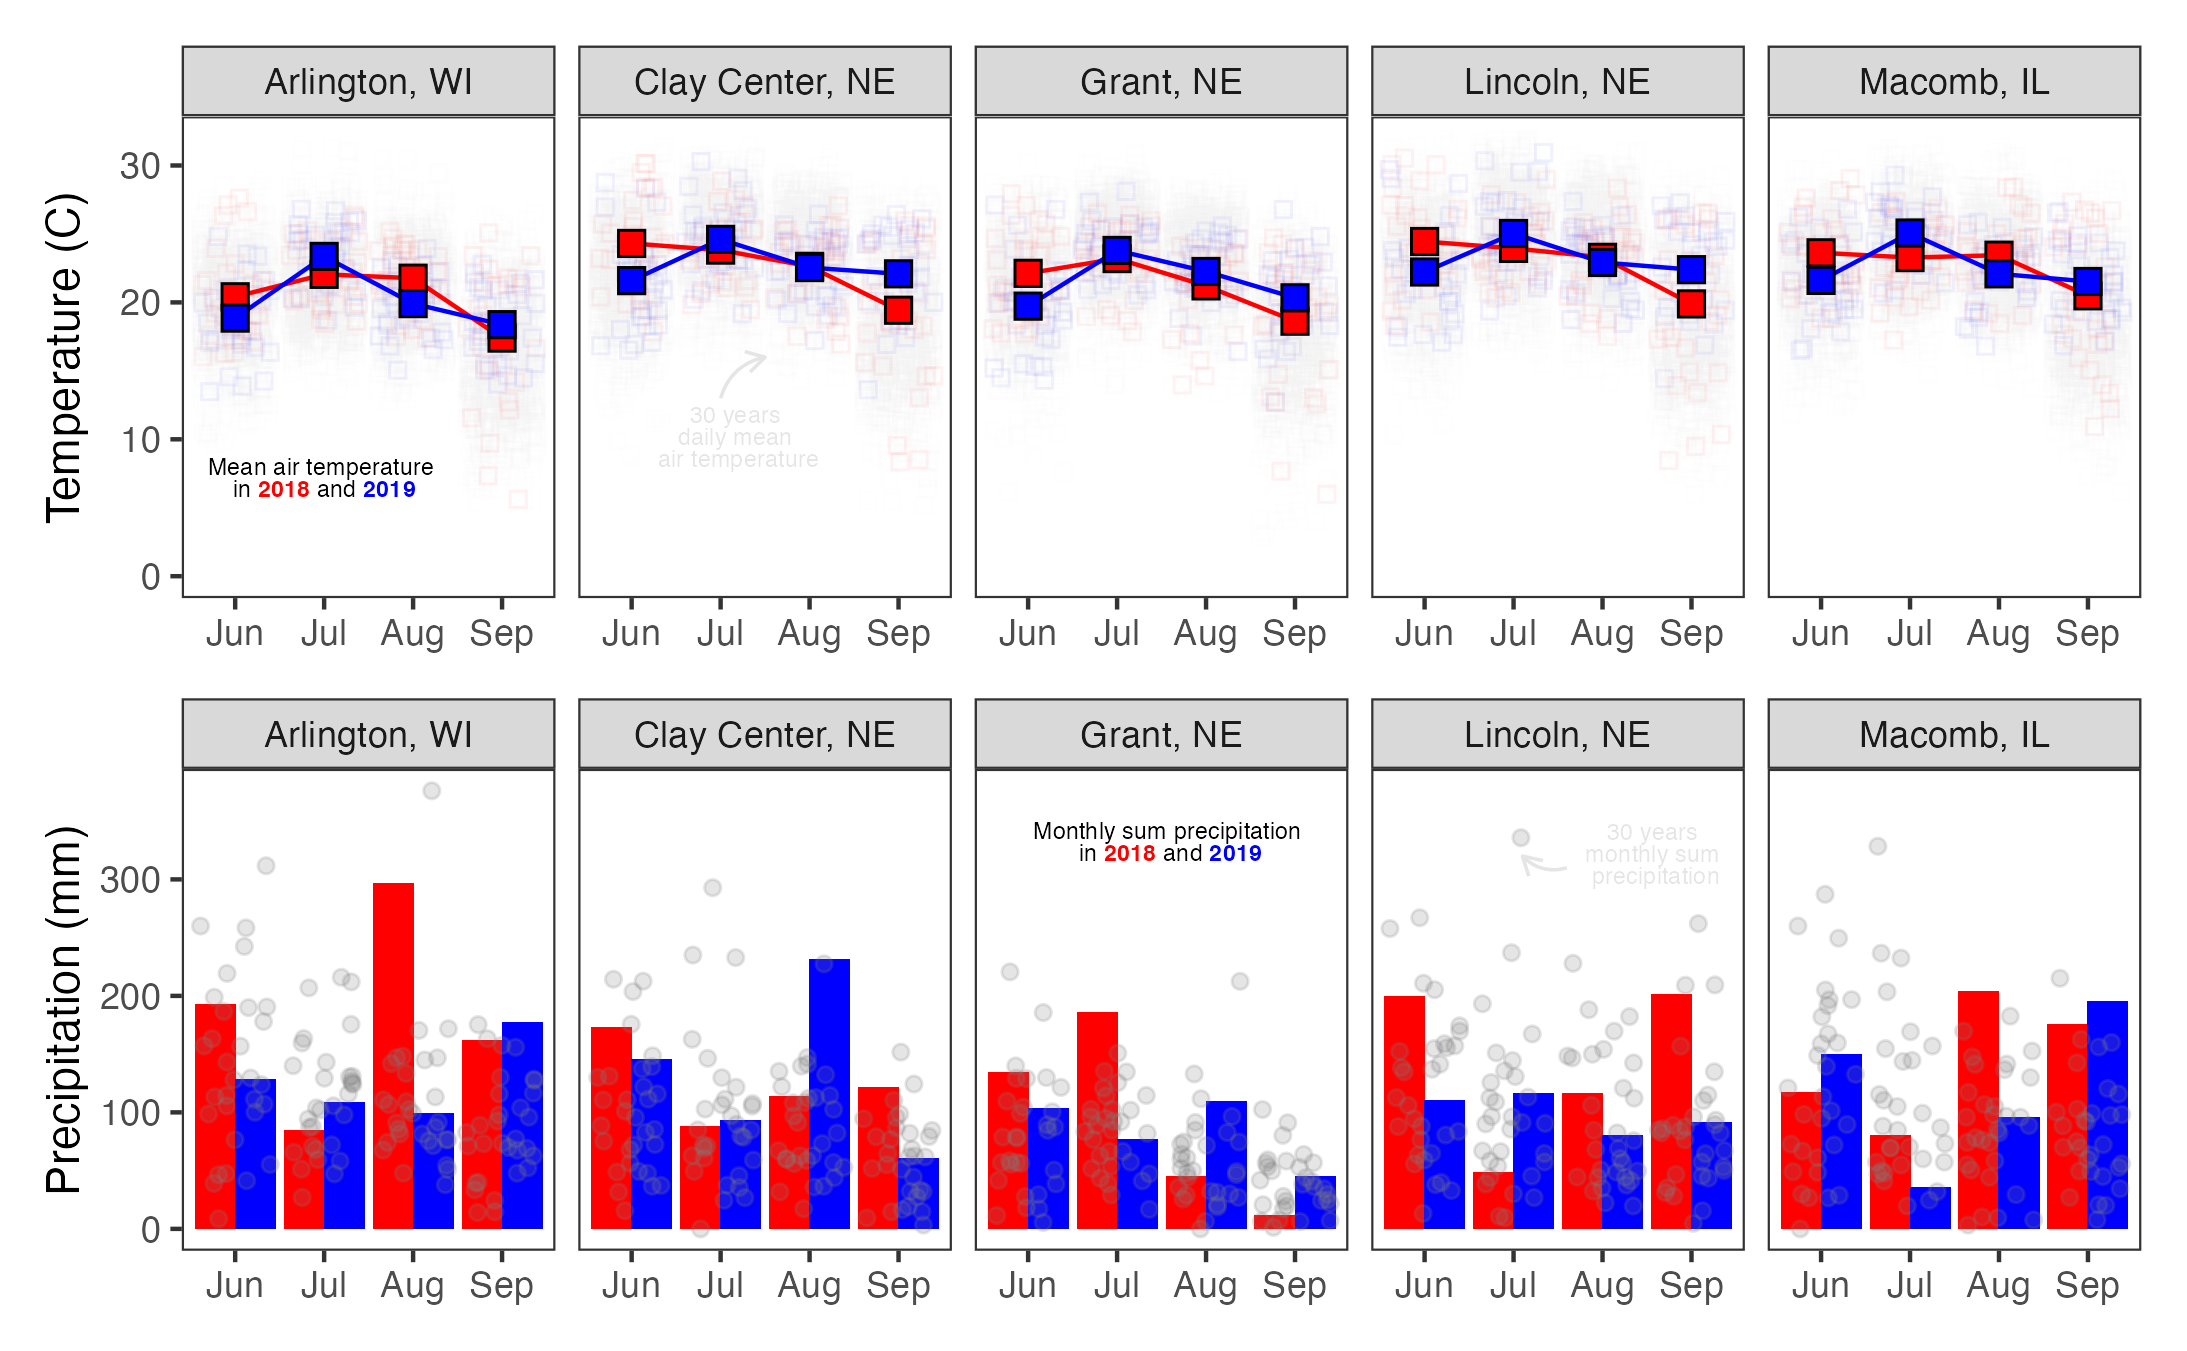
\includegraphics[width=160mm,height=100mm]{../data analysis/weather/Figure 1} 

}

\caption{Mean average temperature (C) and montly sum precipitation (mm) at Arlington, WI, Clay Center, NE, Grant, NE, Lincoln, NE and Macomb, IL}\label{fig:Figure-1}
\end{figure}

\begin{figure}

{\centering 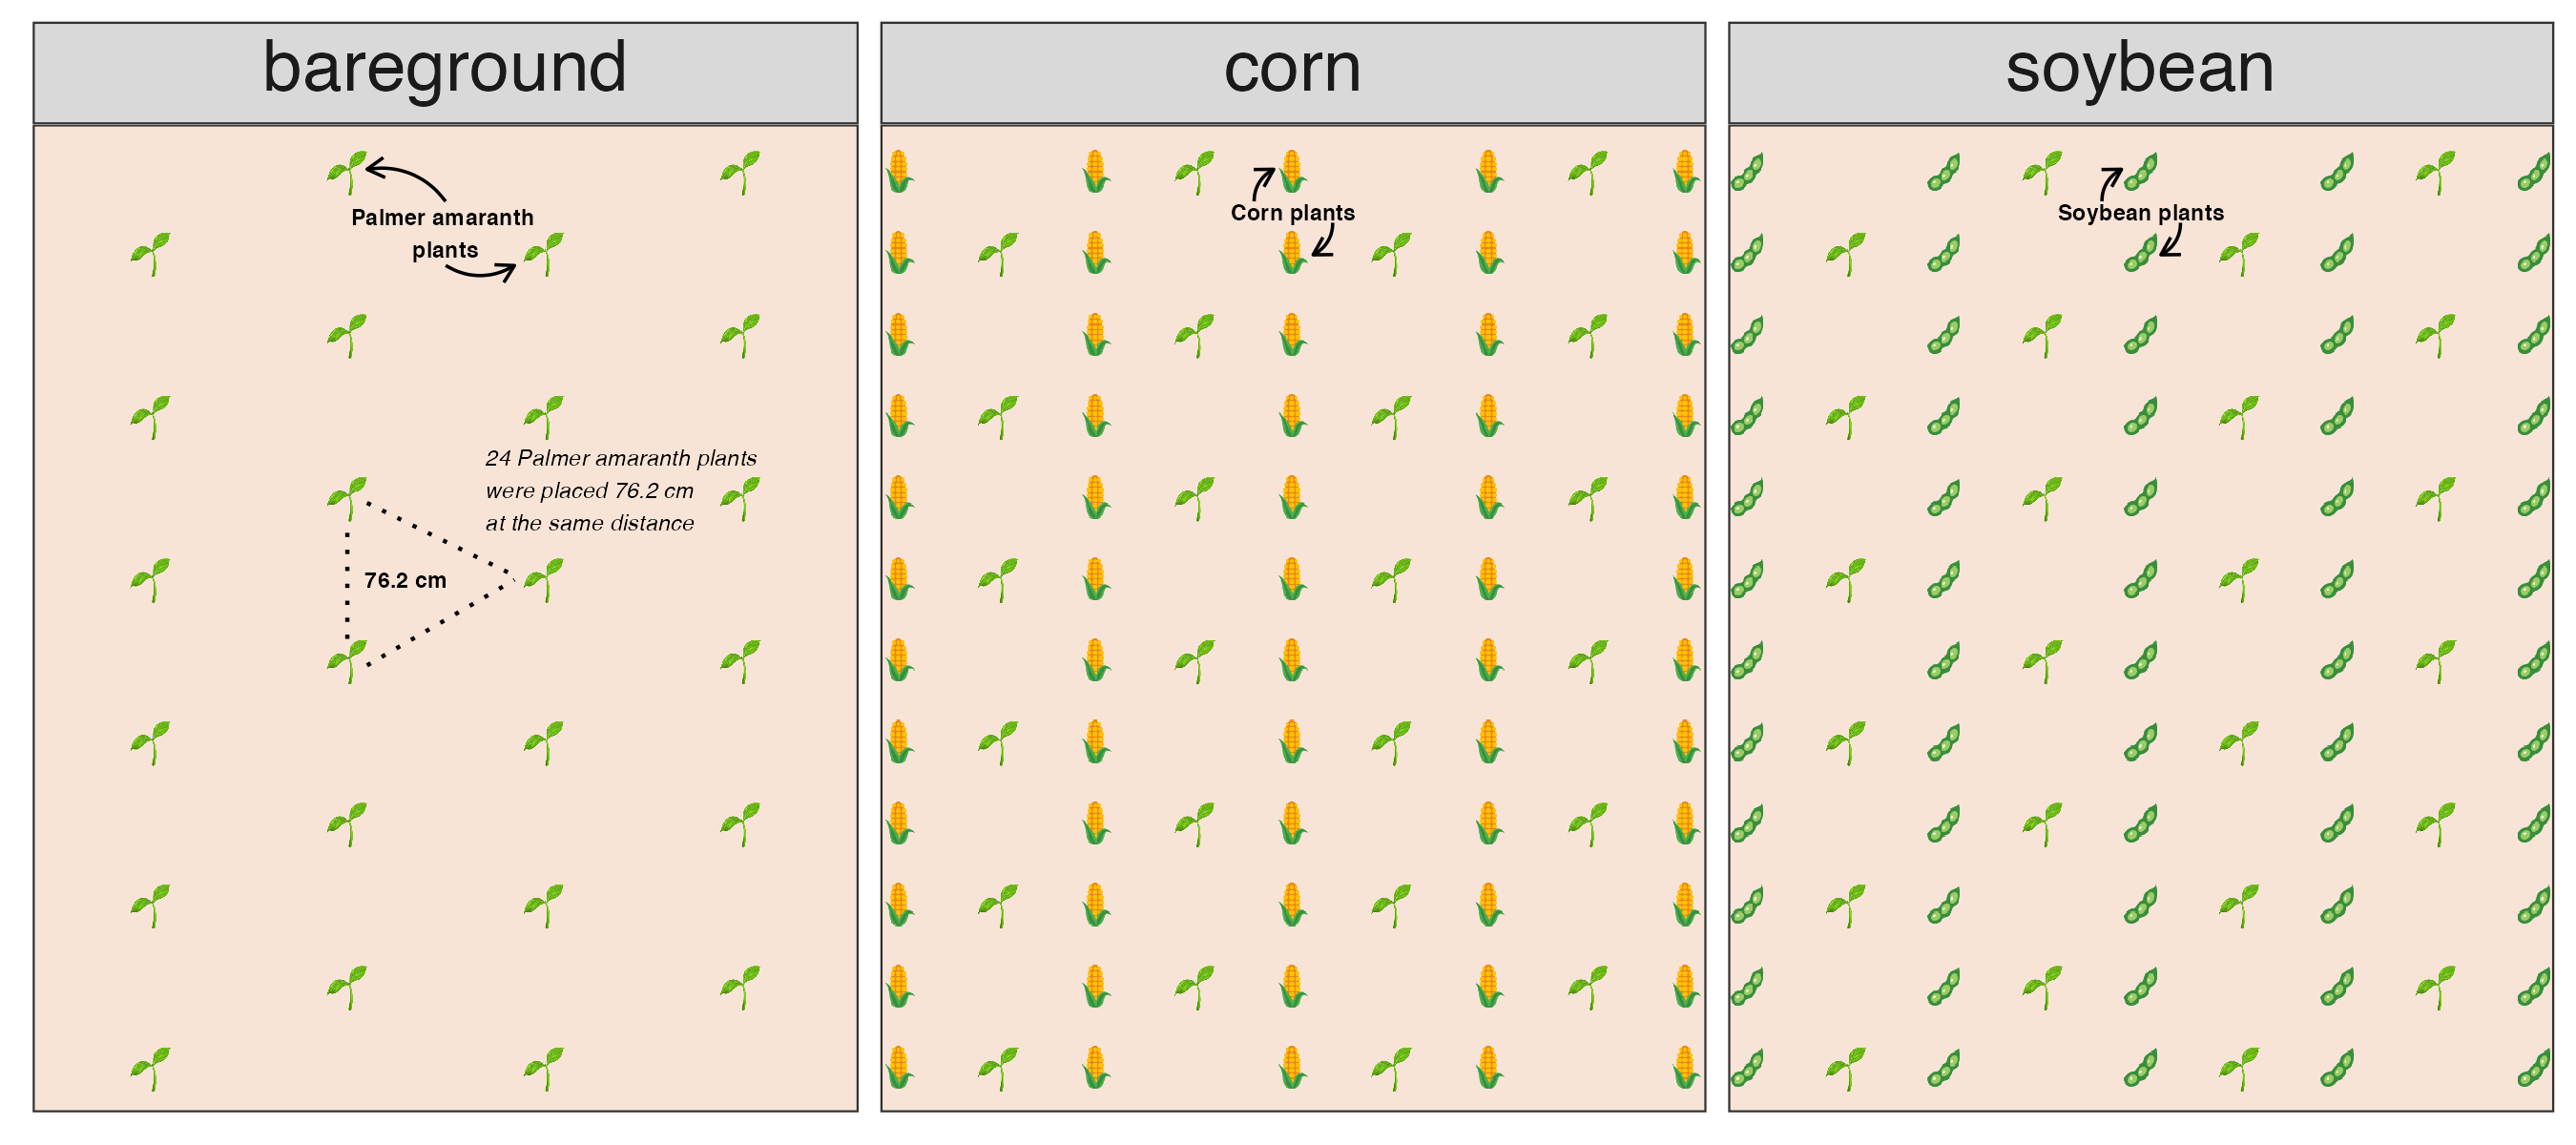
\includegraphics[width=130mm,height=130mm]{../data analysis/figures/Figure 2} 

}

\caption{Cumulative flowering of Palmer amaranth at first and second transplant timing (A) and day of year of 10, 50, and 90 cumulative flowering at first and second transplant timing (B)}\label{fig:Figure-2}
\end{figure}

\begin{figure}

{\centering \includegraphics[width=130mm,height=70mm]{../data analysis/figures/Figure 3} 

}

\caption{Palmer amaranth biomass (A) and height (B) growing in corn, fallow, and soybean across Arlington, Clay Center, Grant, Lincoln, and Macomb}\label{fig:Figure-3}
\end{figure}

\begin{figure}

{\centering 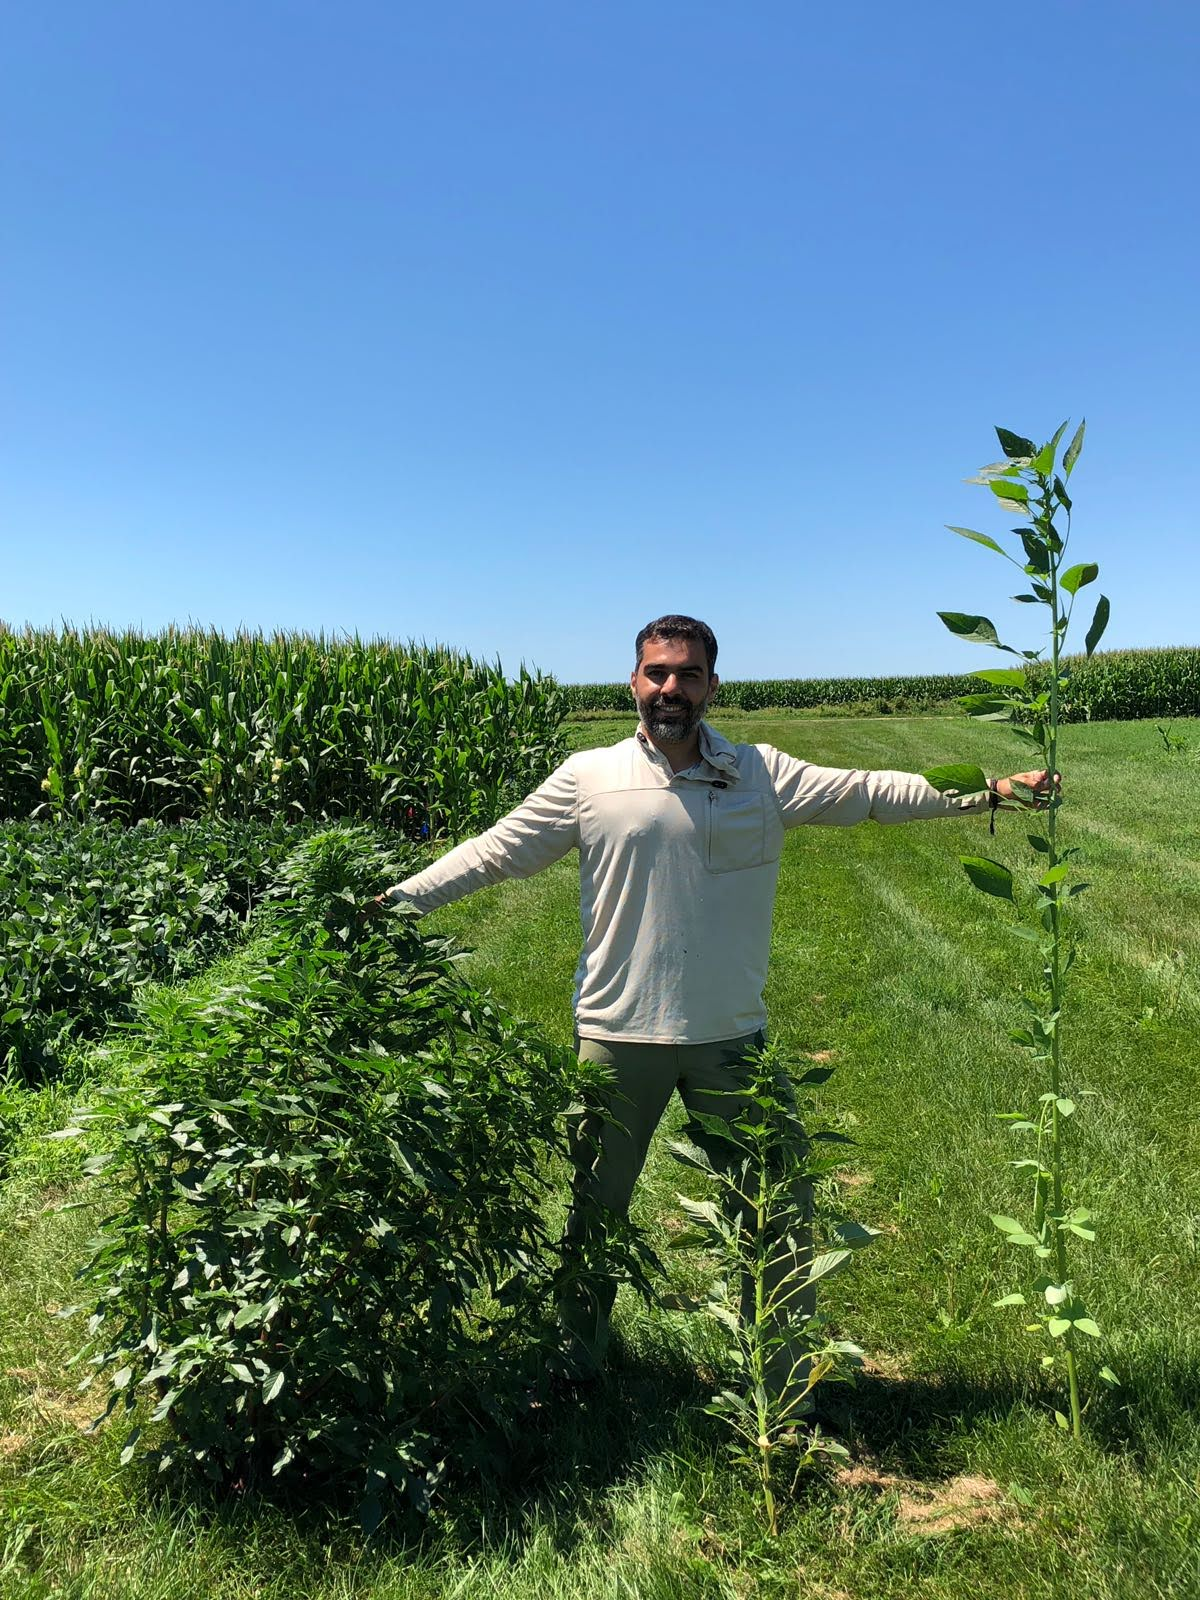
\includegraphics[width=70mm,height=70mm]{../data analysis/figures/image} 

}

\caption{Harvest Palmer amaranth plants at 40 days after first transplant timing. From left to right, Palmer amaranth growing in fallow, soybean and corn in Arlington, Wisconsin}\label{fig:Figure-4}
\end{figure}

\hypertarget{refs}{}
\begin{CSLReferences}{1}{0}
\leavevmode\hypertarget{ref-aulakh2021}{}%
Aulakh, J. S., Chahal, P. S., Kumar, V., Price, A. J., and Guillard, K.
(2021). Multiple herbicide-resistant {Palmer} amaranth ({Amaranthus}
palmeri) in {Connecticut}: Confirmation and response to {POST}
herbicides. \emph{Weed Technology} 35, 457--463.
doi:\href{https://doi.org/10.1017/wet.2021.6}{10.1017/wet.2021.6}.

\leavevmode\hypertarget{ref-bagavathiannan2016}{}%
Bagavathiannan, M. V., and Norsworthy, J. K. (2016). Multiple-{Herbicide
Resistance Is Widespread} in {Roadside Palmer Amaranth Populations}.
\emph{PLOS ONE} 11, e0148748.
doi:\href{https://doi.org/10.1371/journal.pone.0148748}{10.1371/journal.pone.0148748}.

\leavevmode\hypertarget{ref-bates2015}{}%
Bates, D., Mächler, M., Bolker, B., and Walker, S. (2015). Fitting
{Linear Mixed}-{Effects Models Using} Lme4. \emph{Journal of Statistical
Software} 67, 1--48.
doi:\href{https://doi.org/10.18637/jss.v067.i01}{10.18637/jss.v067.i01}.

\leavevmode\hypertarget{ref-berger2015}{}%
Berger, S. T., Ferrell, J. A., Rowland, D. L., and Webster, T. M.
(2015). Palmer {Amaranth} ({Amaranthus} palmeri) {Competition} for
{Water} in {Cotton}. \emph{Weed Science} 63, 928--935.
doi:\href{https://doi.org/10.1614/WS-D-15-00062.1}{10.1614/WS-D-15-00062.1}.

\leavevmode\hypertarget{ref-briscoerunquist2019}{}%
Briscoe Runquist, R. D., Lake, T., Tiffin, P., and Moeller, D. A.
(2019). Species distribution models throughout the invasion history of
{Palmer} amaranth predict regions at risk of future invasion and reveal
challenges with modeling rapidly shifting geographic ranges. \emph{Sci
Rep} 9, 2426.
doi:\href{https://doi.org/10.1038/s41598-018-38054-9}{10.1038/s41598-018-38054-9}.

\leavevmode\hypertarget{ref-chahal2018}{}%
Chahal, P. S., Irmak, S., Jugulam, M., and Jhala, A. J. (2018).
Evaluating {Effect} of {Degree} of {Water Stress} on {Growth} and
{Fecundity} of {Palmer} amaranth ({Amaranthus} palmeri) {Using Soil
Moisture Sensors}. \emph{Weed Science} 66, 738--745.
doi:\href{https://doi.org/10.1017/wsc.2018.47}{10.1017/wsc.2018.47}.

\leavevmode\hypertarget{ref-correndo2021}{}%
Correndo, A. A., Moro Rosso, L. H., and Ciampitti, I. A. (2021).
Retrieving and processing agro-meteorological data from {API}-client
sources using {R} software. \emph{BMC Research Notes} 14, 205.
doi:\href{https://doi.org/10.1186/s13104-021-05622-8}{10.1186/s13104-021-05622-8}.

\leavevmode\hypertarget{ref-farmer2017}{}%
Farmer, J. A., Webb, E. B., Pierce, R. A., and Bradley, K. W. (2017).
Evaluating the potential for weed seed dispersal based on waterfowl
consumption and seed viability. \emph{Pest Management Science} 73,
2592--2603. doi:\href{https://doi.org/10.1002/ps.4710}{10.1002/ps.4710}.

\leavevmode\hypertarget{ref-fox2018}{}%
Fox, J., and Weisberg, S. (2018). \emph{An {R Companion} to {Applied
Regression}}. {SAGE Publications} Available at:
\url{http://books.google.com?id=uPNrDwAAQBAJ}.

\leavevmode\hypertarget{ref-garetson2019}{}%
Garetson, R., Singh, V., Singh, S., Dotray, P., and Bagavathiannan, M.
(2019). Distribution of herbicide-resistant {Palmer} amaranth
({Amaranthus} palmeri) in row crop production systems in {Texas}.
\emph{Weed Technology} 33, 355--365.
doi:\href{https://doi.org/10.1017/wet.2019.14}{10.1017/wet.2019.14}.

\leavevmode\hypertarget{ref-guo2003}{}%
Guo, P., and Al-Khatib, K. (2003). Temperature effects on germination
and growth of redroot pigweed ({Amaranthus} retroflexus), {Palmer}
amaranth ({A}. Palmeri), and common waterhemp ({A}. rudis). \emph{Weed
Science} 51, 869--875.
doi:\href{https://doi.org/10.1614/P2002-127}{10.1614/P2002-127}.

\leavevmode\hypertarget{ref-hartzler2016}{}%
Hartzler, B., and Anderson, M. (2016). Palmer amaranth: {It}'s here, now
what? 10.

\leavevmode\hypertarget{ref-heap2021}{}%
Heap, I. (2021). Internation {Herbicide}-{Resistant Weed Database}.
Available at: \url{http://www.weedscience.org/Home.aspx} {[}Accessed
July 26, 2021{]}.

\leavevmode\hypertarget{ref-hothorn2008}{}%
Hothorn, T., Bretz, F., and Westfall, P. (2008). Simultaneous
{Inference} in {General Parametric Models}. \emph{Biometrical Journal}
50, 346--363.
doi:\href{https://doi.org/10.1002/bimj.200810425}{10.1002/bimj.200810425}.

\leavevmode\hypertarget{ref-jha2010}{}%
Jha, P., Norsworthy, J. K., Riley, M. B., and Bridges, W. (2010). Annual
{Changes} in {Temperature} and {Light Requirements} for {Germination} of
{Palmer Amaranth} ({Amaranthus} palmeri) {Seeds Retrieved} from {Soil}.
\emph{Weed Science} 58, 426--432.
doi:\href{https://doi.org/10.1614/WS-D-09-00038.1}{10.1614/WS-D-09-00038.1}.

\leavevmode\hypertarget{ref-keeley1987}{}%
Keeley, P. E., Carter, C. H., and Thullen, R. J. (1987). Influence of
{Planting Date} on {Growth} of {Palmer Amaranth} ({Amaranthus} palmeri).
\emph{Weed Science} 35, 199--204.
doi:\href{https://doi.org/10.1017/S0043174500079054}{10.1017/S0043174500079054}.

\leavevmode\hypertarget{ref-kistner2018}{}%
Kistner, E. J., and Hatfield, J. L. (2018). Potential {Geographic
Distribution} of {Palmer Amaranth} under {Current} and {Future
Climates}. \emph{Agricultural \& Environmental Letters} 3, 170044.
doi:\href{https://doi.org/10.2134/ael2017.12.0044}{10.2134/ael2017.12.0044}.

\leavevmode\hypertarget{ref-klingaman1994}{}%
Klingaman, T. E., and Oliver, L. R. (1994). Palmer {Amaranth}
({Amaranthus} palmeri) {Interference} in {Soybeans} ({Glycine} max).
\emph{Weed Science} 42, 523--527.
doi:\href{https://doi.org/10.1017/S0043174500076888}{10.1017/S0043174500076888}.

\leavevmode\hypertarget{ref-kohrt2017}{}%
Kohrt, J. R., Sprague, C. L., Nadakuduti, S. S., and Douches, D. (2017).
Confirmation of a {Three}-{Way} ({Glyphosate}, {ALS}, and {Atrazine})
{Herbicide}-{Resistant Population} of {Palmer Amaranth} ({Amaranthus}
palmeri) in {Michigan}. \emph{Weed Science} 65, 327--338.
doi:\href{https://doi.org/10.1017/wsc.2017.2}{10.1017/wsc.2017.2}.

\leavevmode\hypertarget{ref-kupper2017}{}%
Küpper, A., Borgato, E. A., Patterson, E. L., Netto, A. G., Nicolai, M.,
Carvalho, S. J. P. de, Nissen, S. J., Gaines, T. A., and Christoffoleti,
P. J. (2017). Multiple {Resistance} to {Glyphosate} and {Acetolactate
Synthase Inhibitors} in {Palmer Amaranth} ({Amaranthus} palmeri)
{Identified} in {Brazil}. \emph{Weed Science} 65, 317--326.
doi:\href{https://doi.org/10.1017/wsc.2017.1}{10.1017/wsc.2017.1}.

\leavevmode\hypertarget{ref-larran2017}{}%
Larran, A. S., Palmieri, V. E., Perotti, V. E., Lieber, L., Tuesca, D.,
and Permingeat, H. R. (2017). Target-site resistance to acetolactate
synthase ({ALS})-inhibiting herbicides in {Amaranthus} palmeri from
{Argentina}. \emph{Pest Management Science} 73, 2578--2584.
doi:\href{https://doi.org/10.1002/ps.4662}{10.1002/ps.4662}.

\leavevmode\hypertarget{ref-lindsay2017}{}%
Lindsay, K., Popp, M., Norsworthy, J., Bagavathiannan, M., Powles, S.,
and Lacoste, M. (2017). {PAM}: {Decision Support} for {Long}-{Term
Palmer Amaranth} ({Amaranthus} palmeri) {Control}. \emph{Weed
Technology} 31, 915--927.
doi:\href{https://doi.org/10.1017/wet.2017.69}{10.1017/wet.2017.69}.

\leavevmode\hypertarget{ref-maclaren2020}{}%
MacLaren, C., Storkey, J., Menegat, A., Metcalfe, H., and
Dehnen-Schmutz, K. (2020). An ecological future for weed science to
sustain crop production and the environment. {A} review. \emph{Agron.
Sustain. Dev.} 40, 24.
doi:\href{https://doi.org/10.1007/s13593-020-00631-6}{10.1007/s13593-020-00631-6}.

\leavevmode\hypertarget{ref-massinga2001}{}%
Massinga, R. A., Currie, R. S., Horak, M. J., and Boyer, J. (2001).
Interference of {Palmer} amaranth in corn. \emph{Weed Science} 49,
202--208.
doi:\href{https://doi.org/10.1614/0043-1745(2001)049\%5B0202:IOPAIC\%5D2.0.CO;2}{10.1614/0043-1745(2001)049{[}0202:IOPAIC{]}2.0.CO;2}.

\leavevmode\hypertarget{ref-matzrafi2021}{}%
Matzrafi, M., Osipitan, O. A., Ohadi, S., and Mesgaran, M. B. (2021).
Under pressure: Maternal effects promote drought tolerance in progeny
seed of {Palmer} amaranth ({Amaranthus} palmeri). \emph{Weed Science}
69, 31--38.
doi:\href{https://doi.org/10.1017/wsc.2020.75}{10.1017/wsc.2020.75}.

\leavevmode\hypertarget{ref-milani2021}{}%
Milani, A., Panozzo, S., Farinati, S., Iamonico, D., Sattin, M., Loddo,
D., and Scarabel, L. (2021). Recent {Discovery} of {Amaranthus} palmeri
{S}. {Watson} in {Italy}: {Characterization} of {ALS}-{Resistant
Populations} and {Sensitivity} to {Alternative Herbicides}.
\emph{Sustainability} 13, 7003.
doi:\href{https://doi.org/10.3390/su13137003}{10.3390/su13137003}.

\leavevmode\hypertarget{ref-morgan2001}{}%
Morgan, G. D., Baumann, P. A., and Chandler, J. M. (2001). Competitive
{Impact} of {Palmer Amaranth} ({Amaranthus} palmeri) on {Cotton}
({Gossypium} hirsutum) {Development} and {Yield}. \emph{Weed Technology}
15, 408--412.
doi:\href{https://doi.org/10.1614/0890-037X(2001)015\%5B0408:CIOPAA\%5D2.0.CO;2}{10.1614/0890-037X(2001)015{[}0408:CIOPAA{]}2.0.CO;2}.

\leavevmode\hypertarget{ref-oliveira2018}{}%
Oliveira, M. C., Gaines, T. A., Patterson, E. L., Jhala, A. J., Irmak,
S., Amundsen, K., and Knezevic, S. Z. (2018). Interspecific and
intraspecific transference of metabolism-based mesotrione resistance in
dioecious weedy {Amaranthus}. \emph{The Plant Journal} 96, 1051--1063.
doi:\href{https://doi.org/10.1111/tpj.14089}{10.1111/tpj.14089}.

\leavevmode\hypertarget{ref-oliveira2021a}{}%
Oliveira, M. C., Giacomini, D. A., Arsenijevic, N., Vieira, G., Tranel,
P. J., and Werle, R. (2021). Distribution and validation of genotypic
and phenotypic glyphosate and {PPO}-inhibitor resistance in {Palmer}
amaranth ({Amaranthus} palmeri) from southwestern {Nebraska}. \emph{Weed
Technology} 35, 65--76.
doi:\href{https://doi.org/10.1017/wet.2020.74}{10.1017/wet.2020.74}.

\leavevmode\hypertarget{ref-page2021}{}%
Page, E. R., Nurse, R. E., Meloche, S., Bosveld, K., Grainger, C.,
Obeid, K., Filotas, M., Simard, M.-J., and Laforest, M. (2021). Import
of {Palmer} amaranth ({Amaranthus} palmeri {S}. {Wats}.) Seed with sweet
potato ({Ipomea} batatas ({L}.) {Lam}) slips. \emph{Can. J. Plant Sci.},
CJPS-2020-0321.
doi:\href{https://doi.org/10.1139/CJPS-2020-0321}{10.1139/CJPS-2020-0321}.

\leavevmode\hypertarget{ref-price2011}{}%
Price, A. J., Balkcom, K. S., Culpepper, S. A., Kelton, J. A., Nichols,
R. L., and Schomberg, H. (2011). Glyphosate-resistant {Palmer} amaranth:
{A} threat to conservation tillage. \emph{Journal of Soil and Water
Conservation} 66, 265--275.
doi:\href{https://doi.org/10.2489/jswc.66.4.265}{10.2489/jswc.66.4.265}.

\leavevmode\hypertarget{ref-ritz2015}{}%
Ritz, C., Baty, F., Streibig, J. C., and Gerhard, D. (2015).
Dose-{Response Analysis Using R}. \emph{PLOS ONE} 10, e0146021.
doi:\href{https://doi.org/10.1371/journal.pone.0146021}{10.1371/journal.pone.0146021}.

\leavevmode\hypertarget{ref-sauer1957}{}%
Sauer, J. (1957). Recent {Migration} and {Evolution} of the {Dioecious
Amaranths}. \emph{Evolution} 11, 11--31.
doi:\href{https://doi.org/10.2307/2405808}{10.2307/2405808}.

\leavevmode\hypertarget{ref-sauer1972}{}%
Sauer, J. D. (1972). The dioecious amaranths: A new species name and
major range extensions. \emph{Madroño} 21, 426--434. Available at:
\url{http://www.jstor.org/stable/41423815}.

\leavevmode\hypertarget{ref-scott2011}{}%
Scott, D. (2011). The {Technological Fix Criticisms} and the
{Agricultural Biotechnology Debate}. \emph{J Agric Environ Ethics} 24,
207--226.
doi:\href{https://doi.org/10.1007/s10806-010-9253-7}{10.1007/s10806-010-9253-7}.

\leavevmode\hypertarget{ref-ward2013}{}%
Ward, S. M., Webster, T. M., and Steckel, L. E. (2013). Palmer
{Amaranth} ({Amaranthus} palmeri): {A Review}. \emph{Weed Technology}
27, 12--27.
doi:\href{https://doi.org/10.1614/WT-D-12-00113.1}{10.1614/WT-D-12-00113.1}.

\leavevmode\hypertarget{ref-yu2021}{}%
Yu, E., Blair, S., Hardel, M., Chandler, M., Thiede, D., Cortilet, A.,
Gunsolus, J., and Becker, R. (2021). Timeline of {Palmer} amaranth
({Amaranthus} palmeri) invasion and eradication in {Minnesota}.
\emph{Weed Technology}, 1--31.
doi:\href{https://doi.org/10.1017/wet.2021.32}{10.1017/wet.2021.32}.

\end{CSLReferences}

\end{document}
